\documentclass{article}
\usepackage[utf8]{inputenc}
\usepackage{geometry}
\usepackage[usenames,dvipsnames,svgnames,table]{xcolor}
%\usepackage{color}
\usepackage{graphicx}
\usepackage[fleqn]{amsmath}
\usepackage{amsfonts}
\usepackage{mathabx}
\usepackage{commath}
\usepackage{bbold}

\geometry{textwidth=6.5in, textheight=9.0in,
    marginparsep=7pt, marginparwidth=.6in}
\setlength{\parindent}{0in}
\setlength{\parskip}{0.08in}

\newcommand{\red}[1]{\textcolor{red}{#1}}
\newcommand{\blue}[1]{\textcolor{blue}{#1}}
\newcommand*{\annot}[1]{\tag*{\footnotesize{\textcolor{gray}{#1}}}}
\newcommand{\like}{\mathcal{L}}
\let\Pr\undefined
\DeclareMathOperator{\R}{R}

\title{Wavefront model}
\author{Josh Meyers}
\date{May 2018}

\begin{document}

\section{Introduction}

We aim to build a model for the HSC field-dependent optics wavefront that can be
trained using out-of-focus ``donut'' images of stars and then used to fit the
optics contribution of in-focus PSFs.  Developing this model is part of our
ongoing effort to factor the PSF into independent contributions from the
atmosphere, optics and sensors.  Such a factorization has many potential
benefits, the greatest of which is likely the ability to capture all of the
effects of CCD-to-CCD discontinuities into the optical component, allowing the
sensor and particularly the atmospheric component to be smoothly interpolated
across the entire field-of-view.  Additional benefits may also include enabling
a significant part of the PSF variation across the field of view to be captured
using just a few parameters, better characterization of high-frequency PSF
components that are not well constrained empirically using finitely sampled
data, and increased ability to characterize the wavelength dependence of the PSF
by characterizing the disparate wavelength dependencies of the individual
components.

\section{Model}

Our model for the optical part of a single star's PSF is Fourier optics.
Specifically, the optical PSF is described by a pupil-obscuration function and
wavefront function. (See DMTN-064 for more details).  Our primary concern for
this note is the spatial variability of the optical wavefront and therefore the
optical PSF over the field of view.  We break down the wavefront model of the
$i$th exposure into three constituent components as follows:

\begin{equation}
    W^i\left(\vec{u}; \vec{\theta}\right) =
    W_\mathrm{tel}\left(\vec{u}; \vec{\theta}\right) +
    W_\mathrm{visit}^i\left(\vec{u}; \vec{\theta}\right) +
    W_\mathrm{CCD}^{\phi_i}\left(\vec{u}; \vec{\theta}\right)
\end{equation}

In the above, $i$ is an index over exposures, $\phi_i$ is the rotator angle for
the $i$th exposure, $\vec{u}$ is a coordinate in the entrance pupil,
$\vec{\theta}$ is the field angle (or equivalently, a location on the focal
plane).  The coordinate system for $\vec{u}$ and $\vec{\theta}$ are understood
to align with the altitude and azimuth axes of the telescope. Note that this
implies that in the presence of a rotator, they are not fixed with respect to
focal plane or CCDs themselves.

The individual terms of the model are:

\begin{itemize}

  \item $W_\mathrm{tel}\left(\vec{u}; \vec{\theta}\right)$  This term is
  intended to model the wavefront perturbations that are present in the
  otherwise unperturbed optical design of the telescope.  It is independent of
  the exposure index $i$, and continuous over the pupil and field of view.

  \item $W_\mathrm{CCD}^{\phi_i}\left(\vec{u}; \vec{\theta}\right)$  This term
  is intended to model wavefront perturbations that are fixed to the CCD array,
  such as may originate from displacements in the heights of each CCD. It is
  continuous in the pupil, but we allow discontinuities between different CCDs
  across the focal plane.  Because this term is constant in focal-plane
  coordinates, but not in our alt-az aligned $\vec{u}$ and $\vec{\theta}$
  coordinates, it also depends on the rotator angle $\phi_i$.  Aside from the
  dependence on $\phi$, this term is constant in time.

  \item $W_\mathrm{visit}^i\left(\vec{u}; \vec{\theta}\right)$  This dynamic
  term is intended to capture exposure-to-exposure differences (beyond the
  rotator angle), that may be due to flexure, temperature variations, or any
  other time-dependent continuous perturbation to the wavefront.  It explicitly
  depends on the exposure index $i$.

\end{itemize}

In DMTN-064, we described how we measured individual wavefronts for a limited
number of pairs of intra- and extra- focal images and specific locations within
the field of view.  For these ``donut'' images, we used a forward model that
decomposed the delivered wavefront into a Zernike polynomial series.  I.e.:

\begin{equation}
    W^i\left(\vec{u}; \vec{\theta}_\ast\right) = \sum_{j=4}^{j_\mathrm{max}} a_j^i(\vec{\theta}_\ast) Z_j(\vec{u})
\end{equation}

In Figure \ref{fig:a69016} we show the field-of-view dependence of such fits to
one exposure.

\begin{figure}
    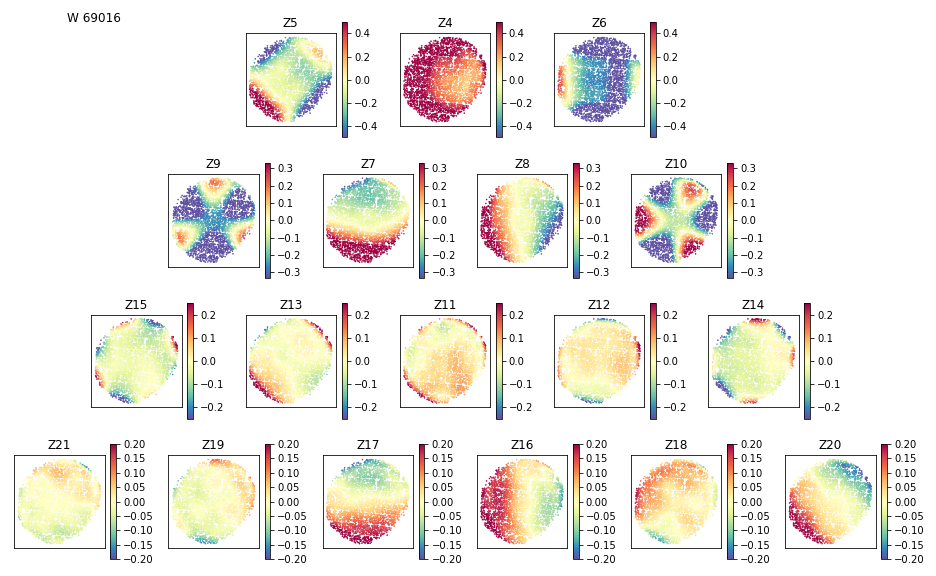
\includegraphics[width=\textwidth]{a69016.png}

    \caption{Zernike coefficient fits for exposure pair 69016/69018.}

    \label{fig:a69016}
\end{figure}

It is useful to apply the same decomposition for the $\vec{u}$ dependence of the
model terms.  I.e., for the telescope and visit terms we will write:

\begin{equation}
    W_\mathrm{tel}\left(\vec{u}; \vec{\theta}\right) =
    \sum_j b^\mathrm{tel}_j (\vec{\theta}) Z_j(\vec{u})
\end{equation}

\begin{equation}
    W^i_\mathrm{visit}\left(\vec{u}; \vec{\theta}\right) =
    \sum_j c^i_j (\vec{\theta}) Z_j(\vec{u})
\end{equation}

We will write the CCD term using focal plane coordinates $\vec{u}^\prime$ and
$\vec{\theta}^\prime$ (instead of alt-az aligned coordinates), since these are
the coordinates in which there is no dependence on the rotator angle $\phi$, and
hence no dependence on the exposure index $i$:

\begin{equation}
    W^\prime_\mathrm{CCD}\left(\vec{u}^\prime; \vec{\theta}^\prime\right) =
    \sum_{j^\prime} d_{j^\prime} (\vec{\theta}^\prime) Z_{j^\prime}(\vec{u}^\prime)
\end{equation}

The trick now is to concretely model the $\vec{\theta}$ dependence which we left
purely abstract above.  For this, we will again use Zernike polynomials, forming
a double zernike basis.  For the telescope and visit terms this becomes:

\begin{equation}
    W_\mathrm{tel}\left(\vec{u}; \vec{\theta}\right) =
    \sum_{jk} b^\mathrm{tel}_{jk} Z_k(\vec{\theta}) Z_j(\vec{u})
    \label{eqn:Wtel}
\end{equation}

\begin{equation}
    W^i_\mathrm{visit}\left(\vec{u}; \vec{\theta}\right) =
    \sum_{jk} c^i_{jk} Z_k(\vec{\theta}) Z_j(\vec{u})
\end{equation}

For the CCD term, we additionally indicate which CCD $n$ the field angle
$\vec{\theta}^\prime$ projects to (using the indicator function
$\mathbb{1}_n(\vec{\theta}^\prime)$):

\begin{equation}
    W^\prime_\mathrm{CCD}\left(\vec{u}^\prime; \vec{\theta}^\prime\right) =
    \sum_{n j^\prime k} d_{n j^\prime k} \mathbb{1}_n(\vec{\theta}^\prime) Z_k(\vec{\theta}^\prime) Z_{j^\prime}(\vec{u}^\prime)
\end{equation}

To incorporate the rotator angle into the last equation, we assert

\begin{equation}
    W^\phi_\mathrm{CCD}\left(\vec{u}; \vec{\theta}\right) =
    W^\prime_\mathrm{CCD}\left(R^\phi\vec{u}; R^\phi\vec{\theta}\right)
\end{equation}

where $R^\phi$ is the normal 2D rotation matrix for angle $\phi$.  For a given
donut or star observation at $\vec{\theta}_\ast$ (in alt-az aligned field
angle), this leads to

\begin{equation}
    W^\phi_\mathrm{CCD}\left(\vec{u}; \vec{\theta}_\ast\right) =
    \sum_{n j^\prime k} d_{n j^\prime k} \mathbb{1}_n(R^\phi \vec{\theta}_\ast) Z_{j^\prime}(R^\phi \vec{u}) Z_k(R^\phi \vec{\theta}_\ast)
\end{equation}

The $Z_k(R^\phi \vec{\theta}_\ast)$ is simply a real number we can compute.  The
$Z_{j^\prime}(R^\phi \vec{u})$ factor is as yet a function here. We will find it
convenient to further decompose it into a series in $Z_j({\vec{u}})$
(eliminating the $R^\phi$) using the mathematics presented in (Tatulli (2013)
arXiv:1302.7106v1).  Namely

\begin{equation}
    Z_{j^\prime}(R^\phi \vec{u}) = \sum_{j} M_{j j^\prime}^\phi Z_{j}(\vec{u})
\end{equation}

where

\begin{equation}
    M_{j j^\prime}^\phi = \delta_{n n^\prime} \times \begin{cases}
    \cos(m \phi), & m = m^\prime \\
    \sin(m \phi), & m = -m^\prime \\
    0 & |m| \ne |m^\prime|
\end{cases}
\end{equation}

where $n$ ($n^\prime$) and $m$ ($m^\prime$) are the radial and azimuthal indices
of the Zernike polynomial with Noll index $j$ ($j^\prime$).  Note that rows or
columns of $M^\phi_{j j^\prime}$ only ever have at most 2 non-zero entries (when
$n = n^\prime$ and $m = \pm m^\prime$).  With this decomposition, we obtain
for each of $W_\mathrm{tel}$, $W_\mathrm{visit}$, and $W_\mathrm{CCD}$ a series
in alt-az aligned pupil Zernikes $Z_j(\vec{u})$.

\section{Donut fits}

\subsection{Formalism}

To determine the unknown coefficients $b^\mathrm{tel}_{jk}$, $c^i_{jk}$, and
$d_{n j^\prime k}$ of our model from a set of pupil Zernike measurements
$\left\{a^*_j\right\}$, we minimize the sum of the least squares residuals $R$
over all of the wavefront measurements:

\begin{equation}
\hspace*{-1cm}
\begin{aligned}
    R\, &\propto \sum_{\ast} \int \dif{\vec{u}} \left\{\mathrm{data} - \mathrm{model}\right\}^2 \\
    &\propto \sum_{\ast}
    \int \dif{\vec{u}} \left\{\sum_j a_j^\ast Z_j(\vec{u})
    - \sum_{jk} b^\mathrm{tel}_{jk} Z_k(\vec{\theta}_\ast) Z_j(\vec{u})
    - \sum_{ijk} \mathbb{1}_i(\ast) c^i_{jk} Z_k(\vec{\theta}_\ast) Z_j(\vec{u})
    - \sum_{injk} \mathbb{1}_n(R^{\phi_i} \vec{\theta}_\ast) \mathbb{1}_i(\ast) \sum_{j^\prime} d_{n j^\prime k} M^{\phi_i}_{j j^\prime} Z_k(R^{\phi_i} \vec{\theta}_\ast) Z_j(\vec{u})
    \right\}^2 \\
    &\propto \sum_{\ast}
    \int \dif{\vec{u}} \left\{\sum_j\left(a_j^\ast
    - \sum_{k} b^\mathrm{tel}_{jk} Z_k(\vec{\theta}_\ast)
    - \sum_{ik} \mathbb{1}_i(\ast) c^i_{jk} Z_k(\vec{\theta}_\ast)
    - \sum_{ink} \mathbb{1}_n(R^{\phi_i} \vec{\theta}_\ast) \mathbb{1}_i(\ast) \sum_{j^\prime} d_{n j^\prime k} M^{\phi_i}_{j j^\prime} Z_k(R^{\phi_i} \vec{\theta}_\ast)
    \right) Z_j(\vec{u})\right\}^2
\end{aligned}
\end{equation}

We use the notation $\mathbb{1}_i(\ast)$ to indicate if a given star was
observed on the $i$th exposure.

Expanding the $\left\{\cdot\right\}^2$ above, we can perform the integral over
$\dif{\vec{u}}$ by taking advantage of the orthogonality of Zernike polynomials:

\begin{equation}
    \int Z_j(\vec{u}) Z_{j^\prime}(\vec{u}) \dif \vec{u} = \pi \delta_{j j^\prime}
\end{equation}

Essentially, only the squares of the terms being indexed by $j$ survive, and all
the cross terms vanish.  This leaves us with

\begin{equation}
    \sum_j \sum_{\ast}
    \left\{a_j^\ast
    - \sum_{k} b^\mathrm{tel}_{jk} Z_k(\vec{\theta}_\ast)
    - \sum_{ik} \mathbb{1}_i(\ast) c^i_{jk} Z_k(\vec{\theta}_\ast)
    - \sum_{ink} \mathbb{1}_n(R^{\phi_i} \vec{\theta}_\ast) \mathbb{1}_i(\ast) \sum_{j^\prime} d_{n j^\prime k} M^{\phi_i}_{j j^\prime} Z_k(R^{\phi_i} \vec{\theta}_\ast)
    \right\}^2
    \label{eqn:loss}
\end{equation}

(with the square now occuring \textit{inside} the summation over $j$).

Although Eq. \ref{eqn:loss} may look complicated, since the terms corresponding
to the model are linear in each of the unknown variables of the model
($b^\mathrm{tel}_{jk}$, $c^i_{jk}$, and $d_{njk}$), we can solve it via standard
linear algebra routines.  Figuratively, we are looking for the least squares
solution to:

\begin{equation}
  \begin{bmatrix}
    \dots & \dots & \dots \\
    \dots & \mathrm{geometry} & \dots \\
    \dots & \dots & \dots
  \end{bmatrix}
  \cdot
  \begin{bmatrix}
    \mathrm{b's} \\
    \dots \\
    \mathrm{c's} \\
    \dots \\
    \mathrm{d's} \\
    \dots
  \end{bmatrix}
  =
  \begin{bmatrix}
    \dots \\
    \mathrm{a's} \\
    \dots
  \end{bmatrix}
  \label{eqn:matrix}
\end{equation}

Also note that the $\{b^\mathrm{tel}_{jk}\}$, and $\{c^i_{jk}\}$ unknown
coefficients only occur in terms that include $a_j^\ast$, i.e., they never occur
in a term that includes $a_{j^\prime}^\ast$ with $j \ne j^\prime$.  Similarly,
the unknown $\{d_{n j^\prime k}\}$ coefficients only occur in terms with at most
one of two different values of $a_j^\ast$, which follows from our earlier
comment that $M^\phi_{j j^\prime}$ only ever has at most 2 non-zero entries per
row or column.  These facts enable us to find the minimum of Eq. \ref{eqn:loss}
in blocks of either 1 or 2 $j$ values at a time.

\subsection{Configuration}

In the above formalism, we never explicitly mentioned the upper indices of the
various summations.  In some cases, these may be fairly obvious, like the upper
index over $i$ is the number of exposure pairs being analyzed, and the upper
index over $n$ is the number of CCDs being analyzed.  In other cases, we
consciously omitted the indices because they are part of the model design --
they're flexible.  For example, the sum over $j$ and $k$ in $W_\mathrm{tel}$
(Eq. \ref{eqn:Wtel}) indicates how much complexity in the pupil (the $j$ index)
and across the field of view (the $k$ index) we want to allow in the
constant-continuous part of the model.  Our intuition for this term from
observing donut fits and from modeling the HSC optics is to allow a large amount
of freedom in the field-of-view dependence of $W_\mathrm{tel}$, and set
$k^\mathrm{max}_\mathrm{tel} = 55$, which is an arbitrary 10th order 2D
polynomial.  The visit term should probably have less freedom than this, as we
expect flexure and temperature fluctuations to induce mostly slowly varying
changes to the wavefront.  We choose $k^\mathrm{max}_{visit} = 10$, which is a
3rd degree polynomial.  For $W_{CCD}$, we only use $k^\mathrm{max}_{CCD} = 1$,
indicating that each CCD only has freedom to change the wavefront by a constant
amount over the CCD.  For each of these terms, we also choose $j^\mathrm{max} =
21$, simply because that's the largest value of $j$ for which we made donut fits
$a_j$.

With the above index upper limits, and using 10 visits and 104 CCDs, our
complete model has 4230 parameters to fit.  We have 20,984 donuts images to
constrain the model, or 377,712 individual $a_j^\ast$ Zernike measurements.

Before we can build the "geometry" matrix of Eqn \ref{eqn:matrix} and fit the
model, we must address one final point, which is that even with many times more
data points than parameters, our model currently has too much freedom to have a
unique best fit solution -- it's degenerate.  For example, increasing the value
of $b^\mathrm{tel}_{4,1}$ is degenerate with either decreasing the values of
each of $c^i_{4,1}$, or decreasing the values of each of $d_{n 4 1}$.  To fix
this, we add the constraint functions

\begin{equation}
  \sum_i c^i_{jk} = 0
\end{equation}

and

\begin{equation}
  \sum_{n} d_{n j^\prime k} = 0
\end{equation}

which select a unique solution from the otherwise infinite set of degenerate
solutions.  The above equations are simply additional rows in the "geometry"
matrix and corresponding 0's added to the "a's" matrix of Eqn. \ref{eqn:matrix}.

In figure \ref{fig:design4}, we show the design matrix for the $j=4$ block of
Eqn. \ref{eqn:loss}.  Each row corresponds to an individual donut measurement
$a^*_4$.  The columns of this design matrix show 3 broad distinct regions, which
correspond from left-to-right with $W_\mathrm{tel}$, $W_\mathrm{CCD}$, and
$W_\mathrm{visit}$.  Within the $W_\mathrm{CCD}$ region, we can see further
subdivisions that correspond to individual CCDs and visits, and within the
$W_mathrm{visit}$ section, we can see individual visits.  In short, the
structure of the design matrix is that every donut constraints $W_\mathrm{tel}$,
constrains the $W_\mathrm{CCD}$ parameters corresponding to the 1 CCD that it
lands on in the 1 visit, and constrains $W_\mathrm{visit}$ parameters that
correspond to its particular visit.

\begin{figure}
    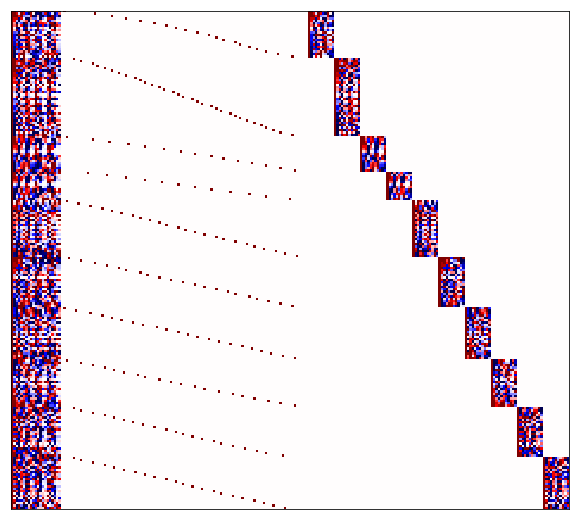
\includegraphics[width=\textwidth]{design4.png}

    \caption{Design matrix for $Z_4$ showing sparse structure.}

    \label{fig:design4}
\end{figure}

In Figure \ref{fig:design56}, we show the design matrix for the combined $j=5$
and $j=6$ block of Eqn. \ref{eqn:loss}.  The same subblocks as in Figure
\ref{fig:design4} are apparent, but doubled.  The doubling is a consequence of
the mixing of $Z_5$ and $Z_6$ under a coordinate system rotation, as discussed
earlier.

\begin{figure}
    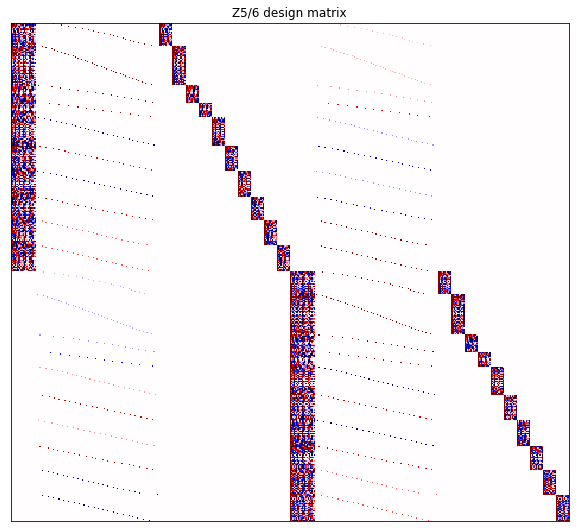
\includegraphics[width=\textwidth]{design56.png}

    \caption{Design matrix for $Z_5$ and $Z_6$ showing how these terms mix
    together.}

    \label{fig:design56}
\end{figure}

\subsection{Fit}

Figures \ref{fig:Wtel}, \ref{fig:WCCD}, and \ref{fig:Wvisit69016} show the
results of fitting the model for $W_\mathrm{tel}$, $W_\mathrm{CCD}$, and for one
particular visit (69016) of $W_\mathrm{visit}$.

$W_\mathrm{tel}$ broadly shows the kinds of patterns that we expect for the
telescope design.  For instance, Zernike terms that vary like $\cos(m \theta)$
in the pupil azimuthal angle $\theta$ vary like $\cos(m \phi)$ in the field
azimuthal angle $\phi$, as must be the case for a circularly symmetric optical
system.  Higher order pupil Zernikes show less amplitude than lower order.

In $W_\mathrm{CCD}$, discontinuities between CCDs are clearly visible (although
note that the amplitudes are pretty small compared to the design amplitudes).
It's worth pointing out that for the circularly symmetric terms (Z4 and Z11),
we expect some degeneracy between $W_\mathrm{tel}$ and $W_\mathrm{CCD}$.  In the
other terms, this degeneracy can largely be broken by simultaneously fitting
exposures taken at different rotator angles.

\begin{figure}
    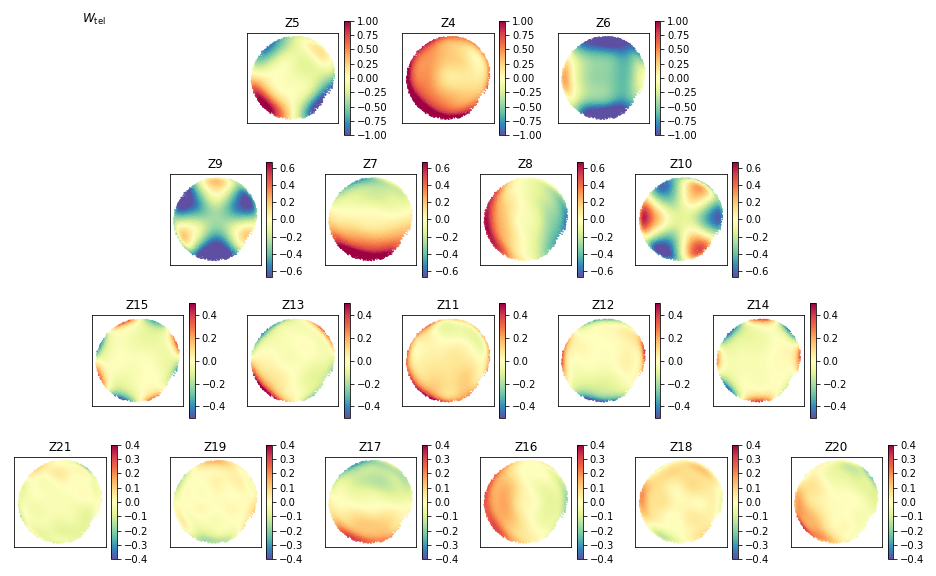
\includegraphics[width=\textwidth]{Wtel.png}

    \caption{$W_\mathrm{tel}$}

    \label{fig:Wtel}
\end{figure}

\begin{figure}
    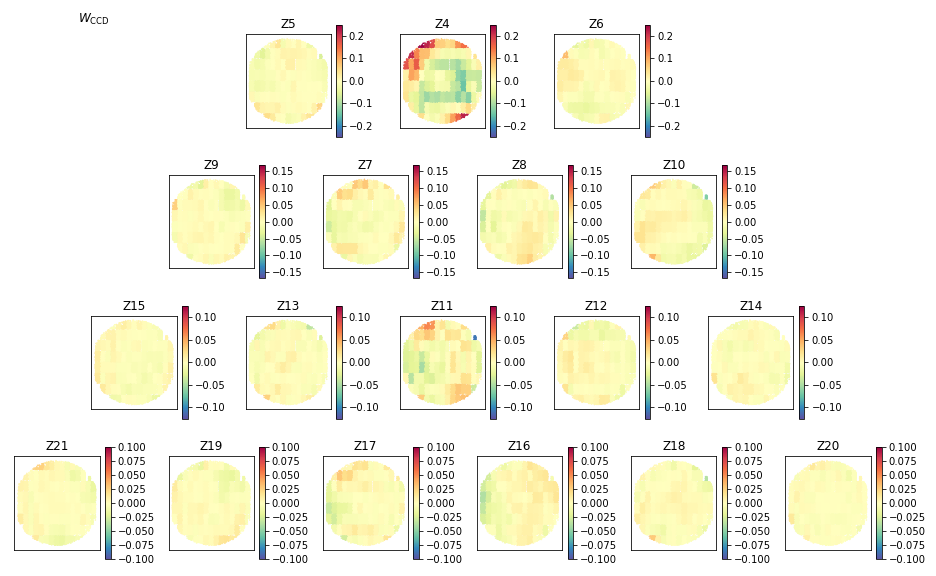
\includegraphics[width=\textwidth]{WCCD.png}

    \caption{$W_\mathrm{CCD}$  Note that the coordinate axes are along the rows
    and columns of the focal plane here.  (And therefore this wavefront figure
    is not aligned with the others in this note.) }

    \label{fig:WCCD}
\end{figure}

\begin{figure}
    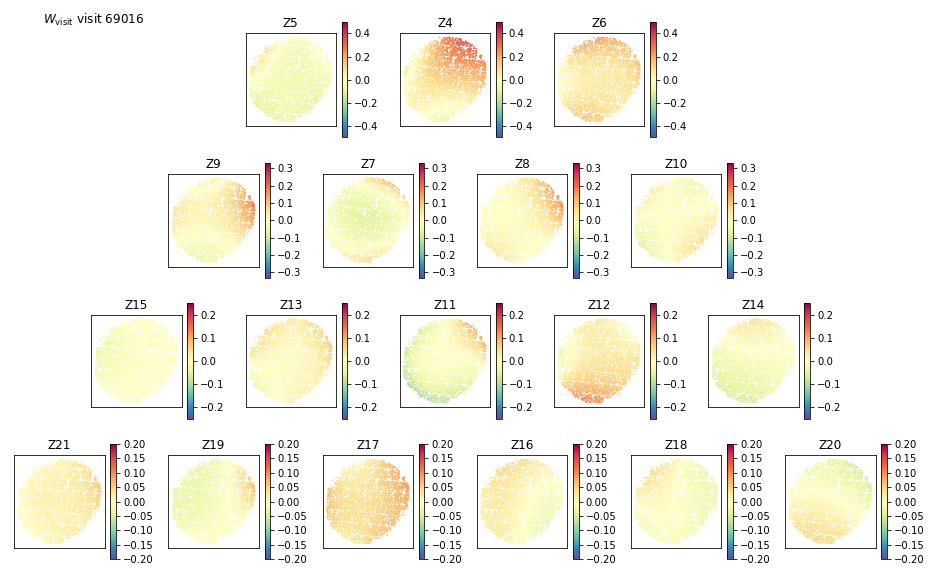
\includegraphics[width=\textwidth]{Wvisit69016.png}

    \caption{$W_\mathrm{visit}$ for exposure pair 69016/69018.}

    \label{fig:Wvisit69016}
\end{figure}

In Figures \ref{fig:W69016} and \ref{fig:Wresid69016} we see the complete model
and the residual.  From the residual plot, it's clear that we've captured most
of the variation in the data.

\begin{figure}
    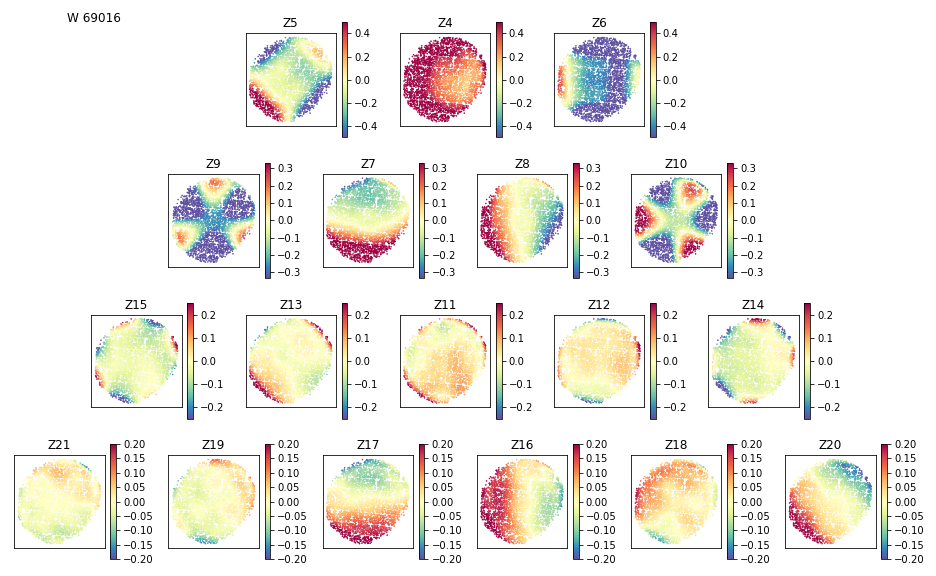
\includegraphics[width=\textwidth]{W69016.png}

    \caption{The complete model for exposure pair 69016/69018.  Note that this
    is \emph{slightly} different than the straight sum of the data in Figures
    \ref{Wtel}, \ref{WCCD}, and \ref{Wvisit69016}, since the $W_\mathrm{CCD}$
    term has been rotated to the particular rotator angle appropriate for this
    exposure pair.}

    \label{fig:W69016}
\end{figure}

\begin{figure}
    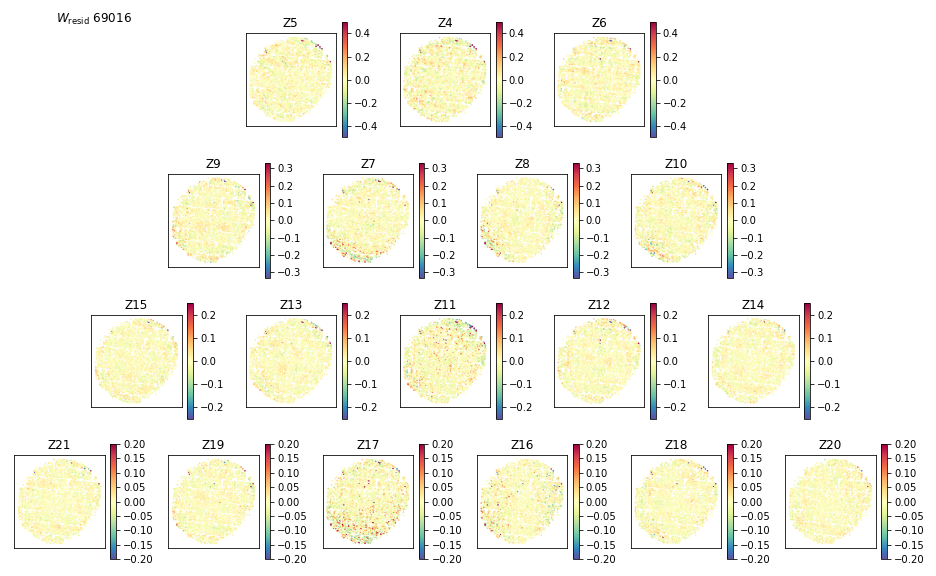
\includegraphics[width=\textwidth]{Wresid69016.png}

    \caption{Residual for exposure pair 69016/69018.  I.e., data (Figure
    \ref{fig:a69016}) minus model (Figure \ref{fig:W69016}).  Aside from
    individual point outliers, there is some barely visible structure in the
    centers of the trefoil (Z9 and Z10) and second astigmatism (Z12 and Z13)
    panels.}

    \label{fig:Wresid69016}
\end{figure}

\section{In-focus fits}

To apply our model to in-focus exposures we A) Fix the values of
$W_\mathrm{tel}$ and $W_\mathrm{CCD}$ found in the preceding analysis (i.e., the
values $b^\mathrm{tel}_{jk}$ and $d_{n j^\prime k}$), and B) apply a
dimensionality reduction to $W_\mathrm{visit}$ (i.e., the values of $c^i_{jk}$).
For B), we specifically use principle component analysis to derive eigen-visits
from the 10 available $W_\mathrm{visit}$ data that we have.  We find that
keeping 3, 4, 5 eigen-visits captures 75\%, 84\%, and 89\% of the variance
amongst all $W_\mathrm{visit}$ terms, respectively.  For the subsequent analysis,
we use 4 eigen-visits.

With the 4 eigen-visits and fixed values of $W_\mathrm{tel}$ and
$W_\mathrm{CCD}$, we can construct a model for the optical part of the PSF
across an entire field of view that only depends on 4 numbers, which are
coefficients of the eigen-visits.

To compare this model to in-focus data, however, we also need to account for the
sensor and atmospheric part of the in-focus PSF (otherwise we'd be comparing
relatively small optics-only PSFs to relatively large optics+atmosphere+sensor
PSFs).  Since we are principally interested in the optics part of the PSF here,
we take a fairly simple model for the atmospheric+sensor PSF, which is a single
elliptical Kolmogorov profile.  This model has three parameters: 1 for the
overall size and 2 for the ellipticity.  Our intention is that this model will
grossly capture the effects of not only the atmosphere, but also the sensors
(charge diffusion) and other PSF contributions not part of the optics, for
example wind shake or tracking errors during the exposure.

The optics + atmoshere + sensor model then contains 7 parameters to optimize for
each exposure: 4 controlling relative amplitudes of the dominant eigen-visits,
and 3 controlling the atmospheric+sensors+etc PSF.

We test this model on a few in-focus exposures.  To fit the model to the data,
we randomly select 100 stars over the field of view and reduce them to their
second moments as measured by HSM.  We do the same for the PSFs predicted by the
model.  We then minimize the sum of the squares of the second moments of all 100
stars.

The results of this in-focus PSF fitting procedure for three different exposures
are presented in Figures \ref{fig:size}, \ref{fig:e1}, and \ref{fig:e2}.  The
PSF sizes and e1 components are relatively well fit by the model.  The e2
components are not particularly well fit; in fact, it appears that there may be
a minus sign error somewhere that is affecting the e2 results.  Overall though,
this approach seems promising in that it can explain are significant part of the
large-field variation of PSF parameters using a very small number of parameters.

\begin{figure}
    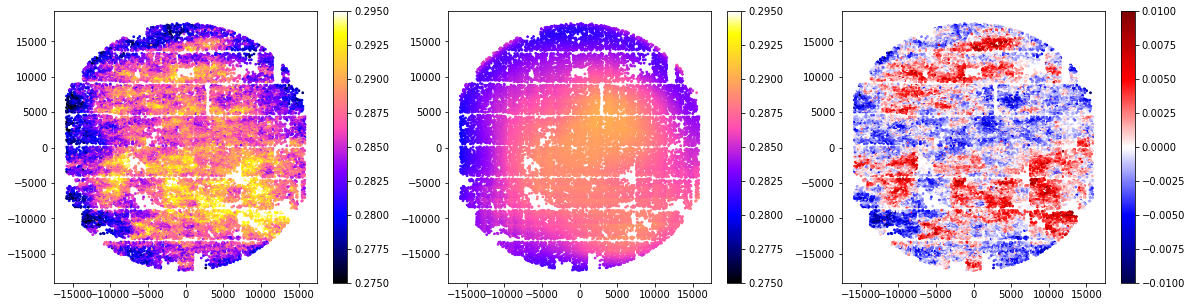
\includegraphics[width=\textwidth]{r_69008.png}
    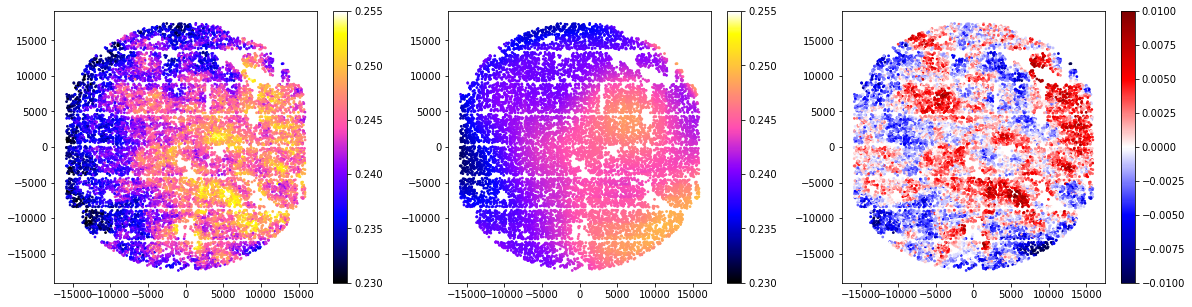
\includegraphics[width=\textwidth]{r_69014.png}
    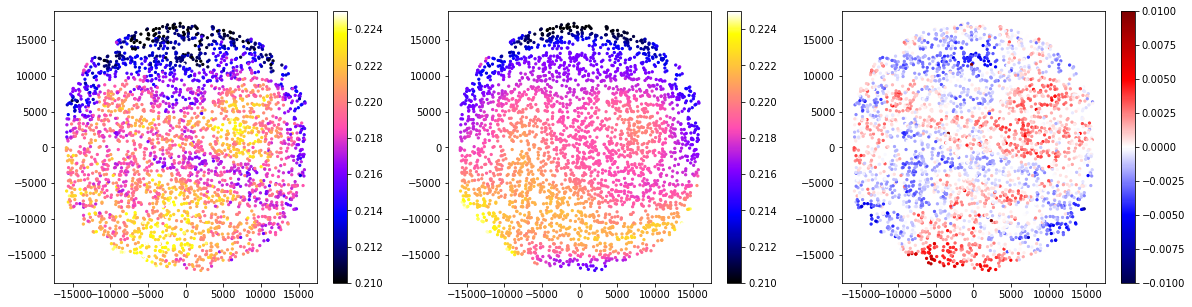
\includegraphics[width=\textwidth]{r_69026.png}

    \caption{PSF sizes.  Different rows correspond to different exposures.  The
    first column are the HSM-measured PSF sizes in the data.  The middle column
    are the best-fit model predictions.  The right column shows the residuals.}

    \label{fig:size}
\end{figure}

\begin{figure}
    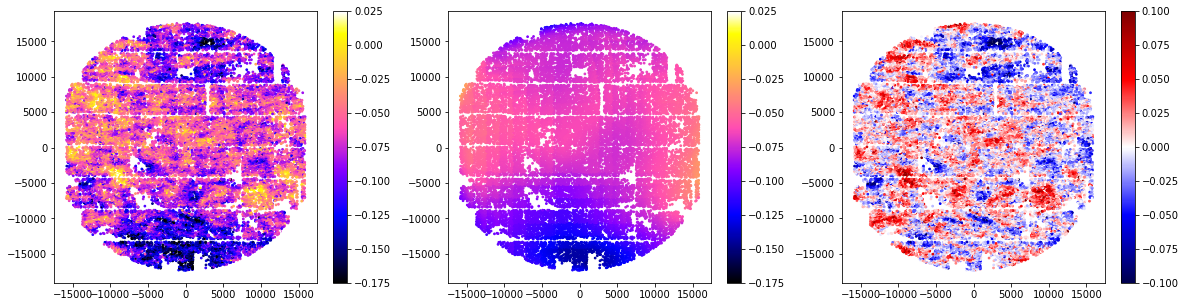
\includegraphics[width=\textwidth]{e1_69008.png}
    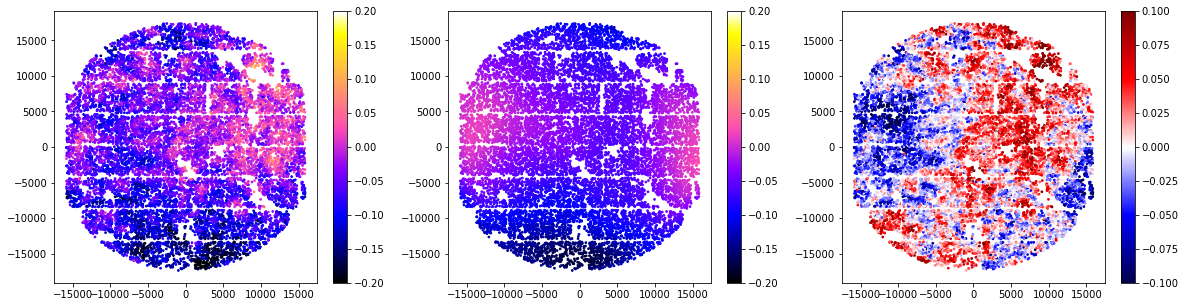
\includegraphics[width=\textwidth]{e1_69014.png}
    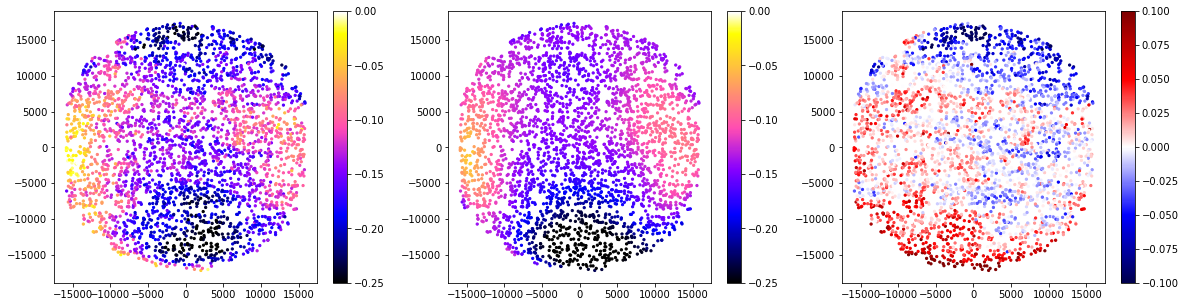
\includegraphics[width=\textwidth]{e1_69026.png}

    \caption{PSF e1 component.  Rows and columns are as in \ref{fig:size}}

    \label{fig:e1}
\end{figure}

\begin{figure}
    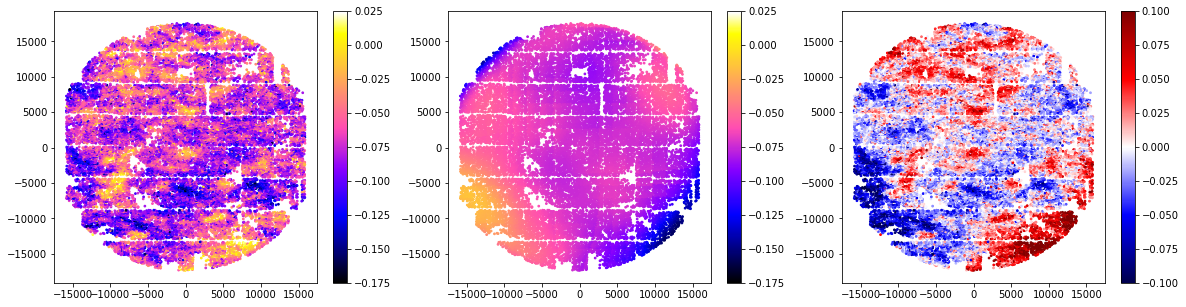
\includegraphics[width=\textwidth]{e2_69008.png}
    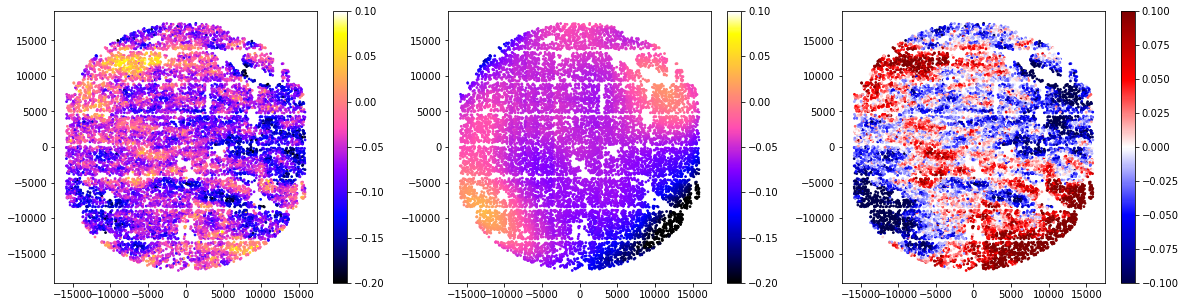
\includegraphics[width=\textwidth]{e2_69014.png}
    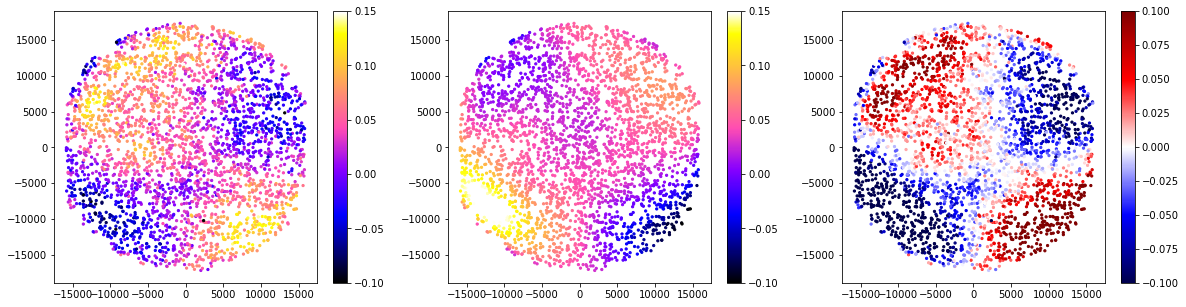
\includegraphics[width=\textwidth]{e2_69026.png}

    \caption{PSF e2 component.  Rows and columns are as in \ref{fig:size}}

    \label{fig:e2}
\end{figure}

\begin{figure}
    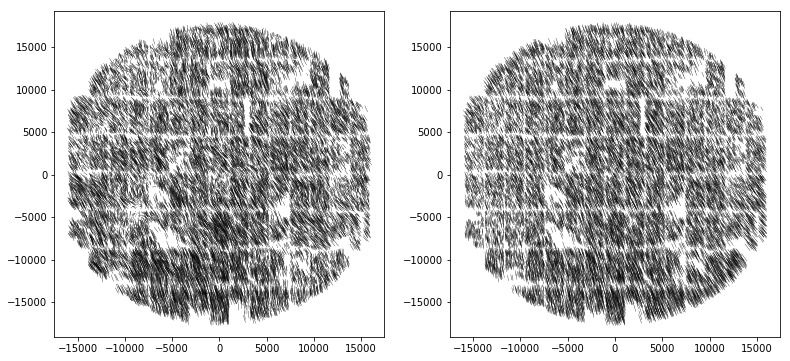
\includegraphics[width=\textwidth]{w_69008.png}
    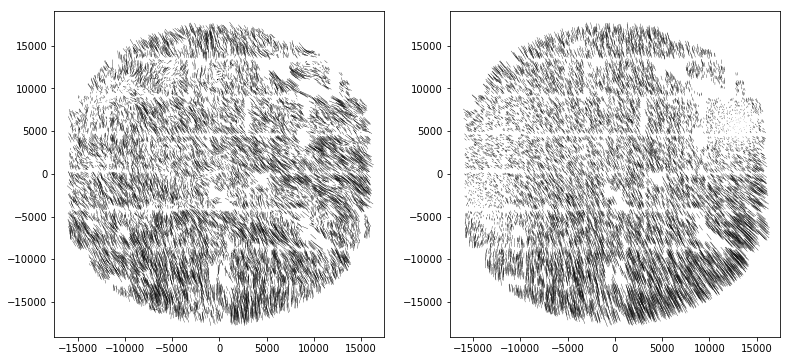
\includegraphics[width=\textwidth]{w_69014.png}
    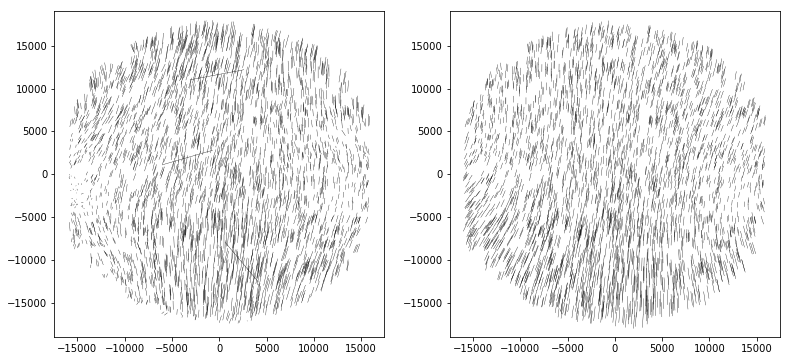
\includegraphics[width=\textwidth]{w_69026.png}

    \caption{PSF whisker comparison.  Rows indicate different exposures.  The
    left column is data, the right column is the best fitting model.}

\end{figure}

\end{document}
